\documentclass[12pt,a4paper,titlepage]{article}

\usepackage{minted}
\usepackage{graphicx}
\usepackage{titlesec}
\usepackage[portuguese]{babel}
\usepackage[colorlinks=true,allcolors=black]{hyperref}

\newcommand{\sectionbreak}{\clearpage}
\graphicspath{ {./img/}{./../../../media/} }
\setminted{
    linenos,
    breaklines=true,
    frame=single,
    style=default
}

\title{Trabalho Prático VI}
\author{
    Fernando de Lima Gonçalves
    \\Fernando Pinto de Queiroz
    \\Henrique Augusto Figueiredo Feydit Vieira
    \\Isabela de Oliveira Miranda
    \\Laura Martins de Souza
    \\Pedro de Castro Dutra Flores
}
\date{Belo Horizonte\\2026}

\begin{document}
\maketitle
\tableofcontents

\clearpage\section{Atividade}
\subsection{Descrição}
"O projeto consiste na simulação do monitoramento do sensor de temperatura utilizado no
trabalho 2. Através do template em Python a ser fornecido, os dados do tópico de temperatura
do trabalho 2 deverão ser armazenados no BD local."

\subsection{Linguagens de Programação}
Para a realização da atividade foram utilizadas as linguagens

\begin{itemize}
    \item \textbf{C/C++:} microcontrolador ESP-32 e envio de dados ao broker.
    \item \textbf{Python:} criação do banco de dados local via coleta de dados no servidor.
    \item \textbf{SQL:} acesso aos dados presentes no banco relacional.
\end{itemize}

\subsection{Banco de Dados}
Para a coleta dos dados foi utilizado um programa em \texttt{Python} capaz de acessar o tópico desejado e popular uma tabela local com os mesmos.
Utilizou-se o banco de dado relacional \texttt{MySQL} em conjunto com a interface \texttt{MySQL Workbench} para visualização dos dados.

\section{Códigos}
\subsection{Microcontrolador: C/C++}
\inputminted{arduino}{../main/main.ino}

\clearpage\subsection{Banco de Dados: Python}
\inputminted{py}{../bd.py}

\clearpage\section{Execução}
\begin{figure}[h]
    \center
    \caption{Banco de Dados TP6 - MySQL Workbench}
    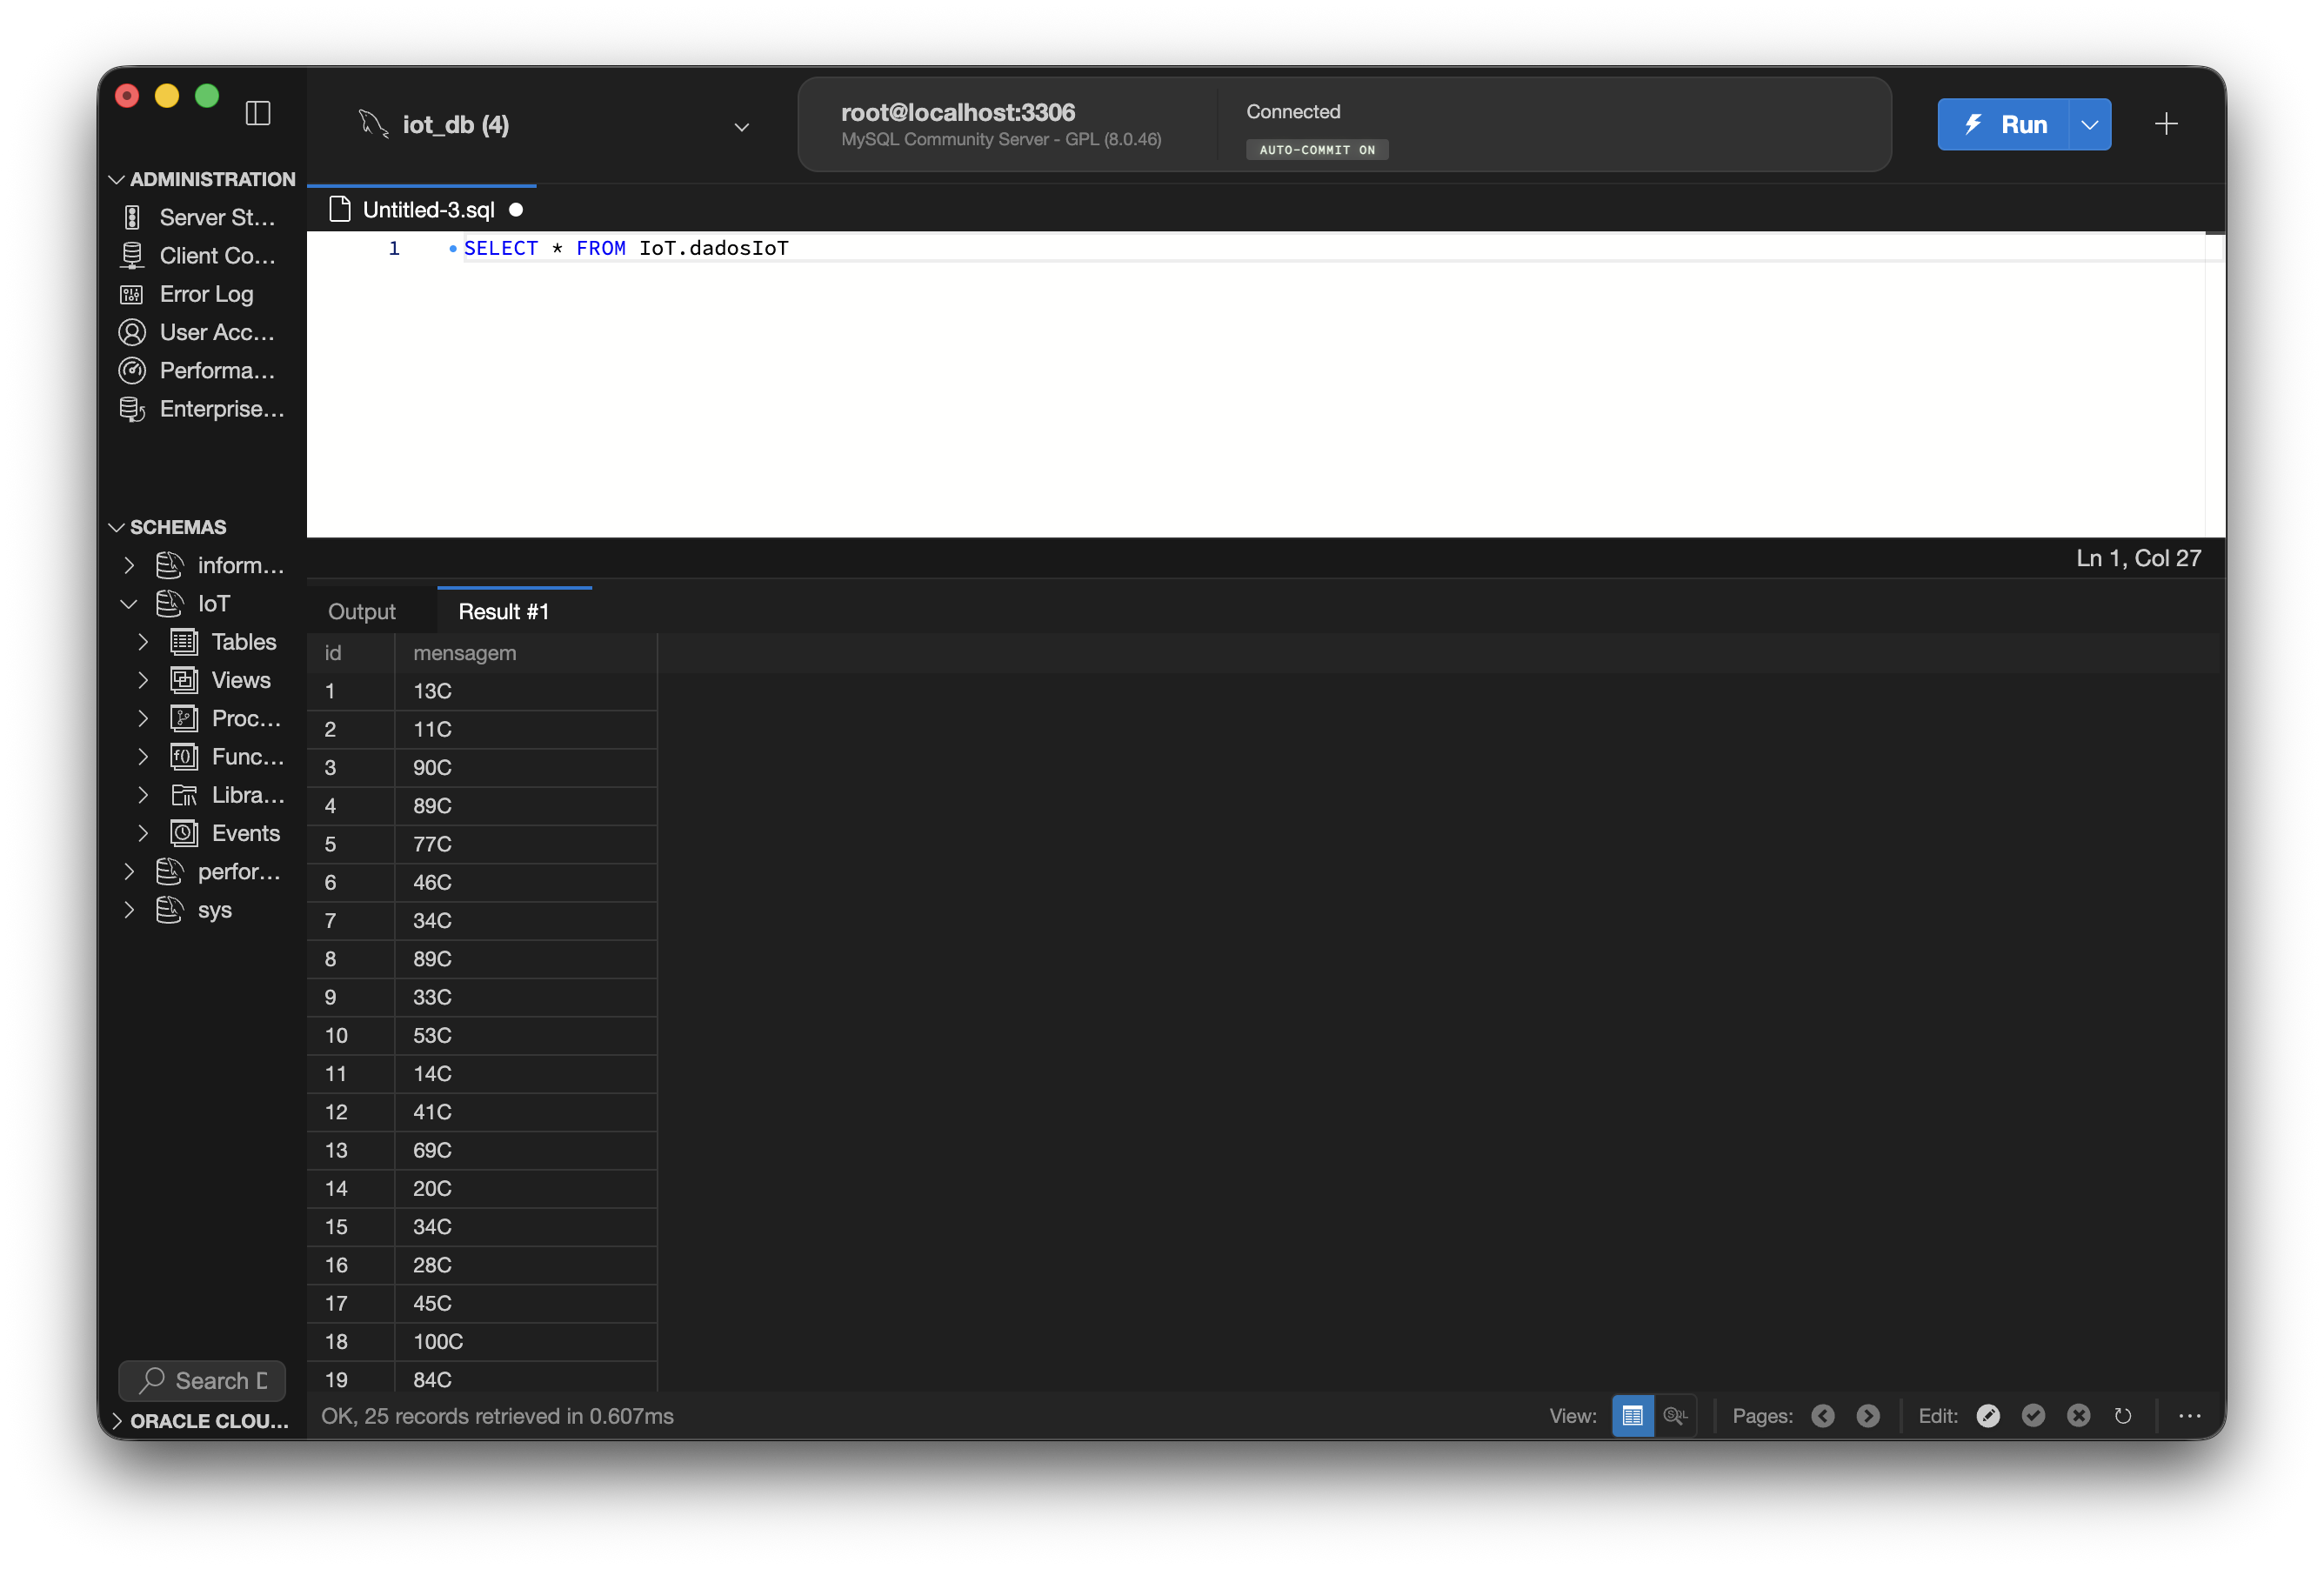
\includegraphics[width=\textwidth]{bd-tp6}
    \par{\small Fonte: Elaborado pelos autores (2026)}
    \label{fig:bd-tp6}
\end{figure}

\end{document}
